\chapter{Nutzung des Backends}
\label{chapter:use}
  
  \section{Einleitung}
  \label{section:backend_introduction}
  
  Über \textbf{bwolf.de/backend} kann das Backend des BWolf-Systems erreicht werden.
  
  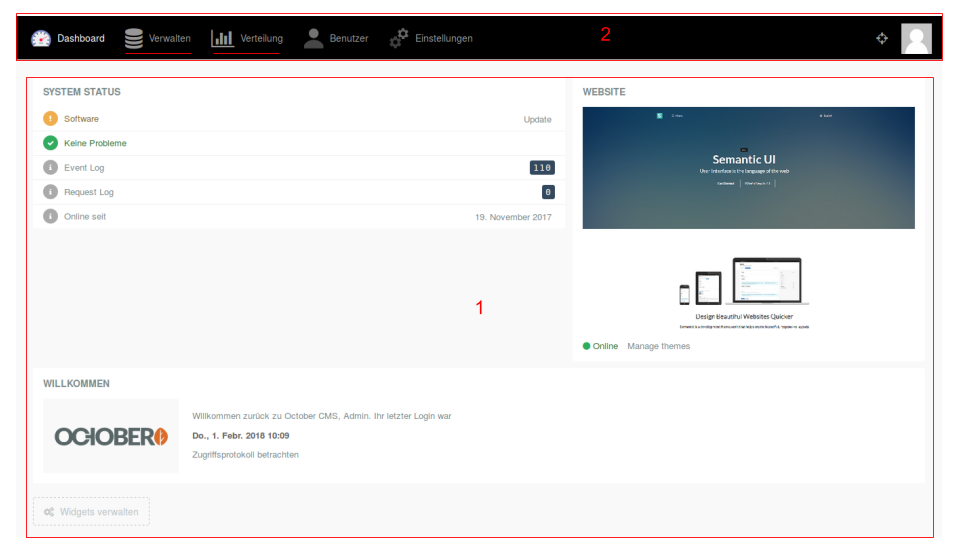
\includegraphics[scale=0.3]{backend/img/dashboard.png}
  %\caption{\newline Der Begrüßungsbildschirm: Das Dashboard aus Sicht des Super-Admins.
%      \newline Normale Administratoren sehen in der oberen Navigation nicht den Punkt ''Benutzer''}
  \begin{enumerate}
   \item Nach der Anmeldung begrüßt das \textbf{Dashboard} den Nutzer. 
	  Hier befinden sich drei Widgets:\newline
	  Bei der Begrüßung befindet sich eine Übersicht über den Systemstatus.\newline
	  Für die elementare Nutzung des Backends, müssen hier keine weiteren Änderungen vorgenommen werden.\newline
	  Sollte in dem Systemstatus ein Problem auftauchen, sollte einer der Entwickler (siehe \textcolor{red}{hier Label Kontakt?}Kontakt)\newline
	  Das Widget \textbf{Website} zeigt an in welchem Theme die Webseite erscheint. Hier sollte auch nichts weiter verändert werden.
	  Ganz zu unterst gibt es noch einen Button \textbf{Widgets verwalten}. 
	  Dieser spielt hier auch keine weitere Rolle, da alle vorhandenen Widgets bereits in das Dashboard integriert wurden.
   \item Über die obere Navigationszeile gelangt der Nutzer zu allen wesentlichen Bereichen des Backends.
	 Zur operativen Benutzung benötigt werden die Bereiche \textbf{Verwalten} und \textbf{Verteilung}
   \item In der oberen Navigationszeile befindet sich ganz rechts die Möglichkeit des Abmeldens.
   \item Das Fadenkreuz daneben ermöglicht es, das Frontend mit den momentan vorgenommenen Einstellungen zu betrachten.
  \end{enumerate}

  
  \section{Verwalten}
  \label{section:manage}
  
    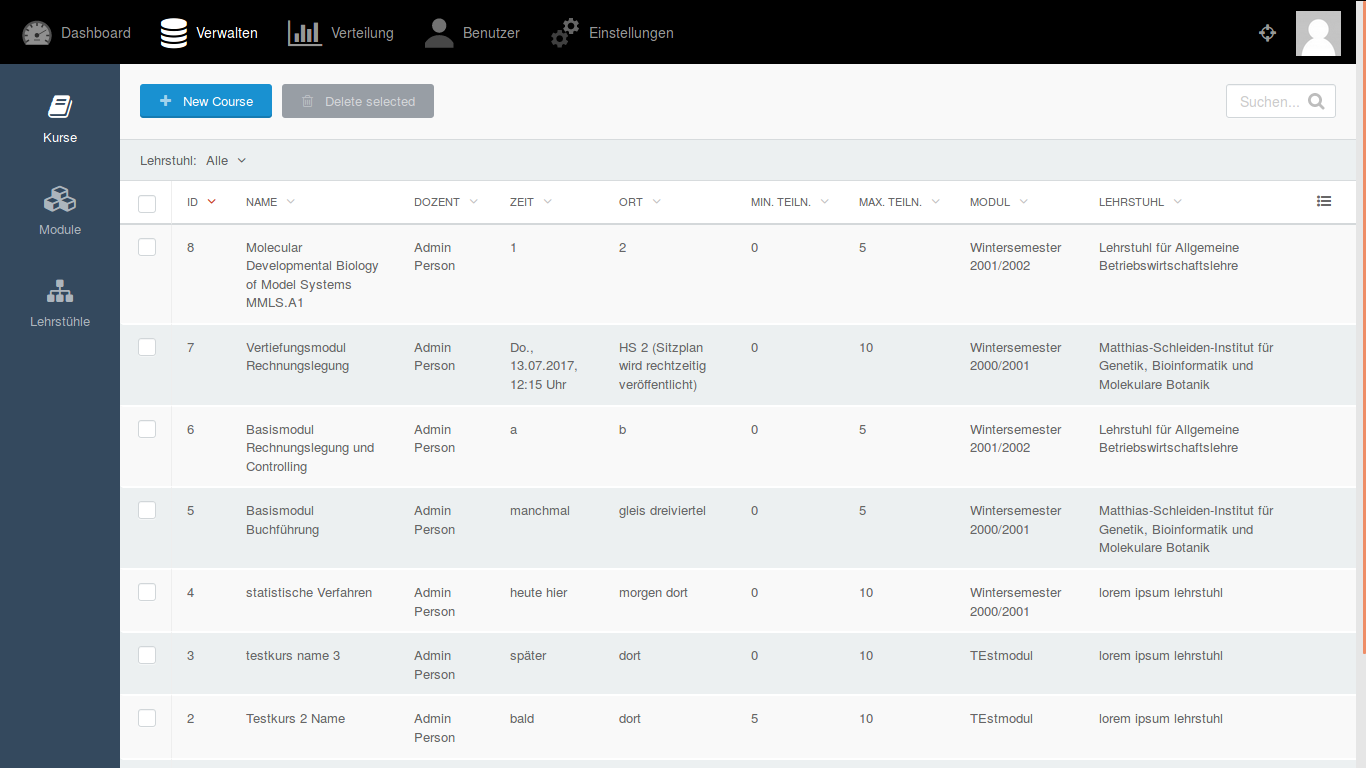
\includegraphics[scale=0.3]{backend/img/verwalten.png}

    In diesem Bereich können der Nutzer neue Module, Lehrstühle und Kurse anlegen.
    Anhand der linken Navigationsspalte können die entsprechenden drei Bereiche erreicht werden.

    In der Übersichtsliste der drei unterschiedlichen Bereiche Module, Lehrstühle und Kurse kann die Reihenfolge der Zeilenelemente durch Betätigen
    der kleinen Pfeile neben den Spaltennamen umsortiert werden.
    In der Kopfzeile dieser Übersichtsliste befindet sich ein Hamburger-Menü. 
    Wenn der Nutzer darauf klickt, öffnet sich ein Popup indem der Nutzer Spalten ein- oder abschalten kann.
    Darüber hinaus kann die maximale Anzahl an Zeileneinträgen pro Seite angegeben werden.
    
    \subsection{Module}
    
    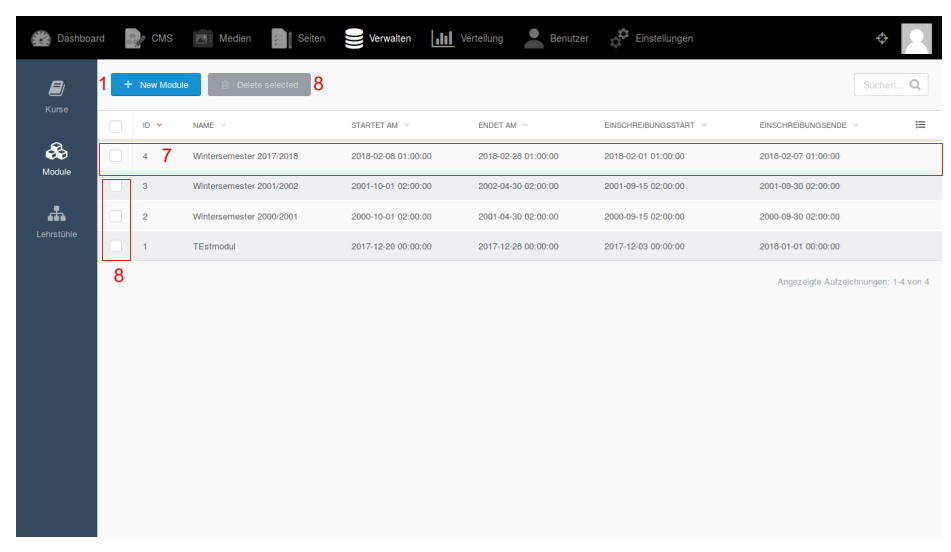
\includegraphics[scale=0.3]{backend/img/module_1.png}

    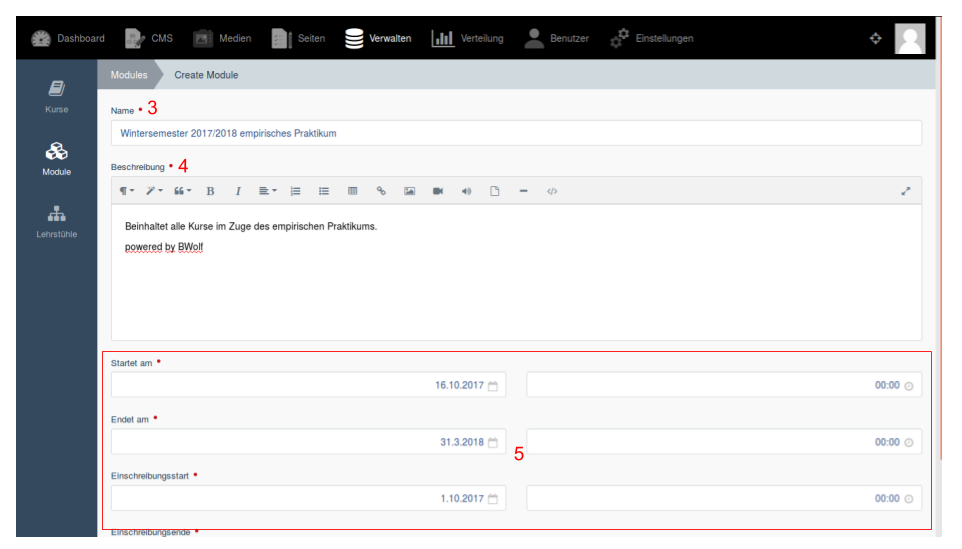
\includegraphics[scale=0.3]{backend/img/module_2.png}

    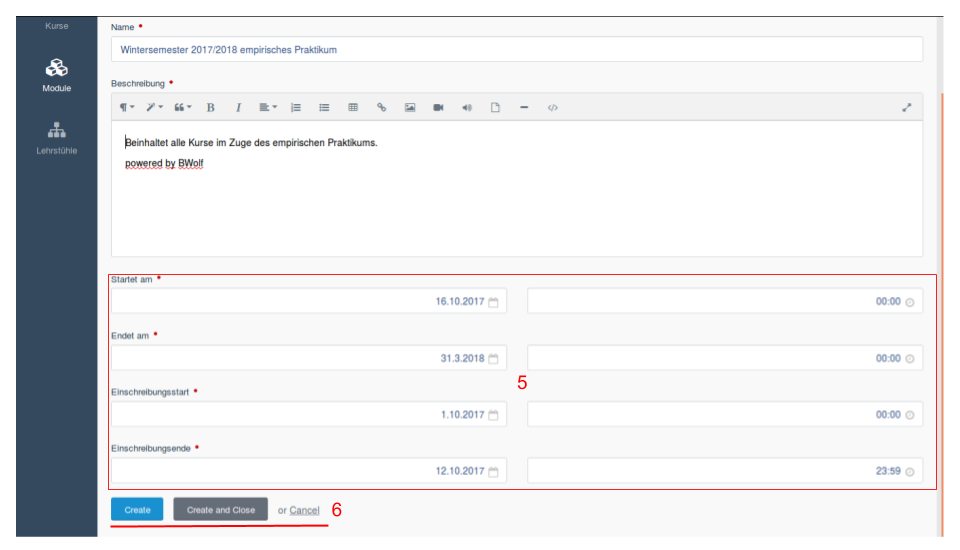
\includegraphics[scale=0.3]{backend/img/module_3.png}
    
    \begin{enumerate}
    \item Zuerst sollte ein neues Modul angelegt werden. Durch Betätigen des \textbf{+ New Module} - Buttons kann ein neuer Kurs angelegt werden.
    \item Hier müssen alle Pflichtfelder - gekennzeichnet durch einen kleinen roten Punkt neben der Feldbeschreibung - ausgefüllt werden.
    \item Ein möglicher Name für einen Modulnamen wäre beispielsweise \textit{Wintersemester 2017/2018 empirisches Praktikum}. Er beschreibt die Veranstaltung.
    \item In den Beschreibungstext können mützliche Informationen zu dem Modul angelegt werden.
	  Hier können neben einfachen Text auch Listen, Bilder, Tabellen und Medienelemente eingefügt werden.
    \item In den Datums- und Zeitfeldern wird der Zeitraum des Moduls angegeben, (beispielsweise 16.10.2017, 00:00 bis 31.03.2018, 23:59) 
	  wie auch der Einschreibungszeitraum in denen sich Studenten für Kurse des Moduls einschreiben können (beispielsweise 1.10.2017, 00:00 bis 12.10.2017, 23:59).
	  Um die Zeitdaten anzugeben, können die aufploppenden Kalender- und Uhrmenüs verwendet werden. Auch die Eingabe über Tastatur ist möglich.
	  Der Einschreibungszeitraum muss vor derm Starttermin des Moduls beginnen.
    \item Über \textbf{Create} wird das neue Modul angelegt. 
	  Durch Betätigen von \textbf{Create and Close} wird das Modul angelegt und der Nutzer landet zurück auf der Übersichtseite aller angelegten Module.
	  Mithilfe von \textbf{Cancel} wird der Erstellungsvorgang abgebrochen.
    \item Durch Anklicken eines der Module kann dieses erneut angepasst werden.
    \item Indem einige Module über die Auswahlkästchen am Beginn der Zeile ausgewählt werden
    \end{enumerate}
    
    \subsection{Lehrstühle}
    
    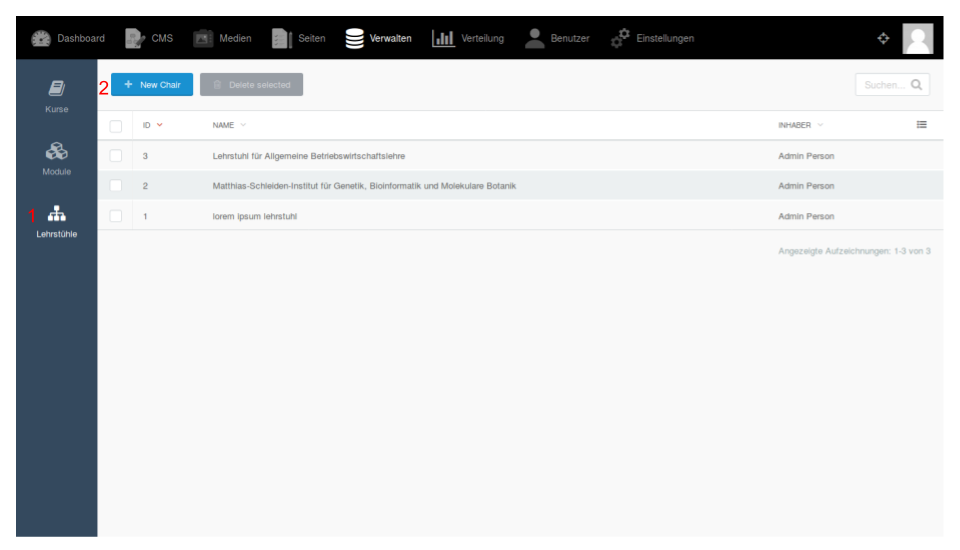
\includegraphics[scale=0.3]{backend/img/chairs_1.png}
    
    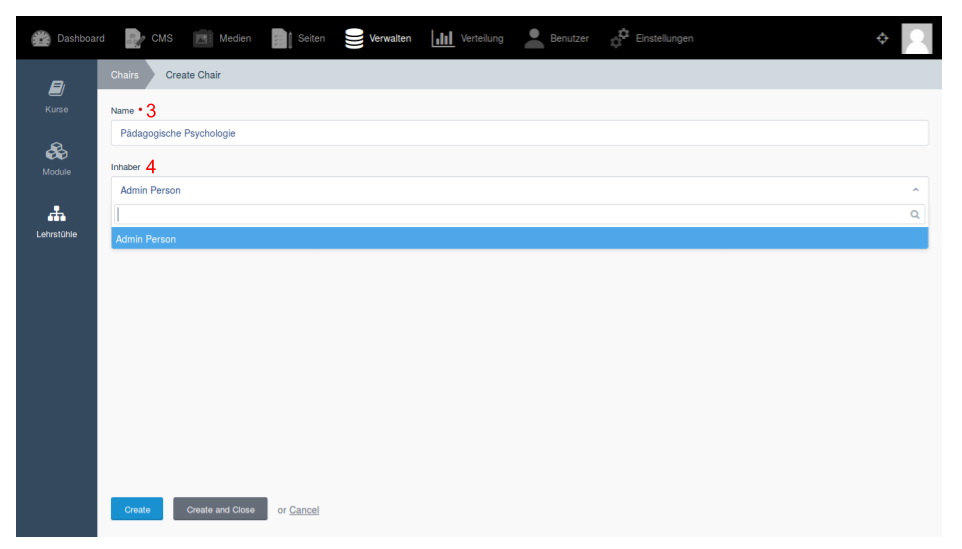
\includegraphics[scale=0.3]{backend/img/chairs_2.png}
    
    \begin{enumerate}
     \item Als nächstes sollten neue Lehrstühle hinzugefügt werden. Dies ist möglich über den dritten Punkt der linken vertikalen Navigation.
     \item Über \textbf{+ New Chair} kann ein neuer Lehrstuhl hinzugefügt werden.
     \item Es muss ein Name vergeben werden. Namensgebung beliebig.
     \item Dem Stuhl kann nur ein Backend-Nutzer zugewiesen werden.
    \end{enumerate}

    \subsection{Kurse}
    
    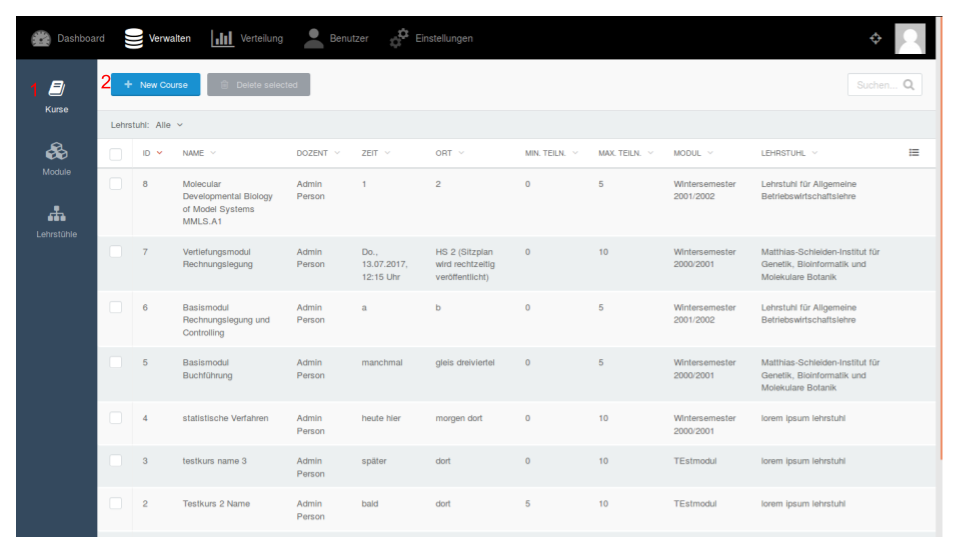
\includegraphics[scale=0.3]{backend/img/verwalten_kurse.png}
    %\caption{Verwalten in der Ansicht ''Kurs''}

    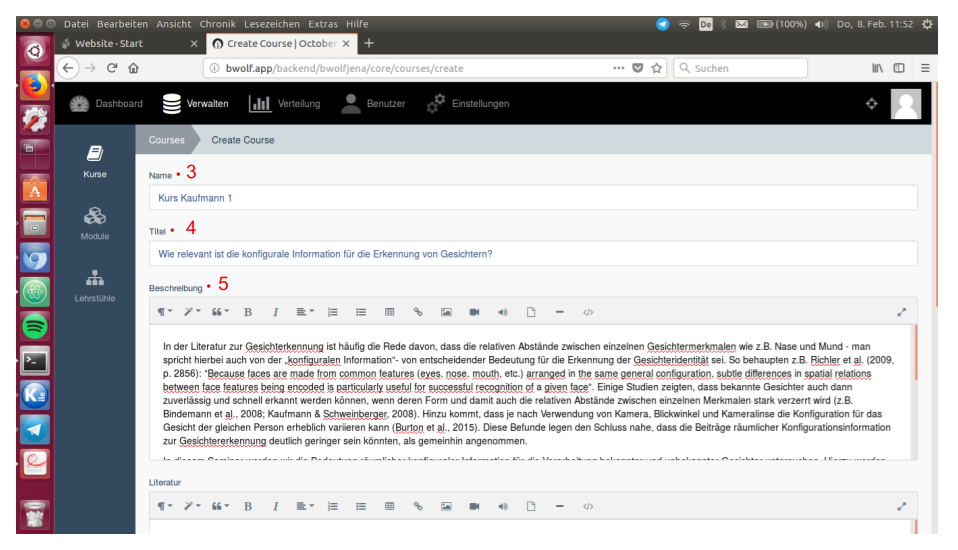
\includegraphics[scale=0.3]{backend/img/create_course_1.png}

    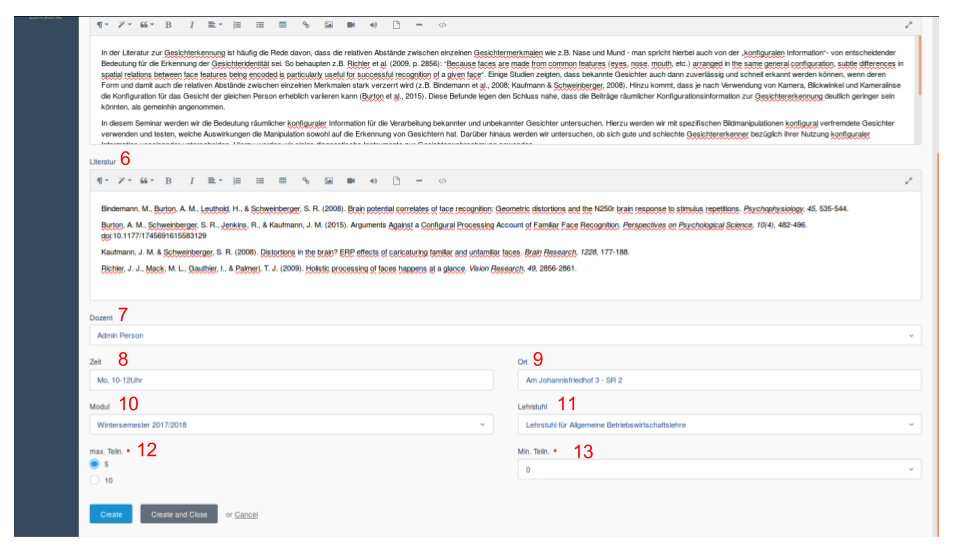
\includegraphics[scale=0.3]{backend/img/create_course_2.png}
    \begin{enumerate}
     \item Über den ersten Punkt der linken Navigation kommt der Nutzer zur Kursübersicht.
     \item In der Kursübersicht kann der Nutzer über \textbf{+ New Course} einen neuen Kurs anlegen.
     \item Ein Kurs benötigt einen Kursnamen. Dieser Name kann zum Beispiel den Namen des Dozenten und evtl eine Zahl beinhalten. Zum Beispiel: \textit{Kurs Kaufmann 1}
     \item In dem Kurstitel sollte dann der eigtl Name des Kurses stehen. Beispielsweise \textit{Wie relevant ist die konfigurale Information für die Erkennung von Gesichtern?}
     \item Die Beschreibung dient als Hilfsmittel zur besseren Beschreibung des Kurses. Sie ist jedoch optional.
	   Hier können rich-text-Elemente wie Tabellen, Bilder und Textbearbeitung dafür genutzt werden.
     \item Als gesonderten Bereich der Beschreibung gibt es die Literatur. Mithilfe einer Ungeordneten Liste kann hier Literatur eingetragen werden.
     \item Über Dozent kann dem Kurs ein verantwortlicher Dozent, bzw. Administrator zugewiesen werden.
     \item In der Zeiteingabe kann ein Text eingegeben werden. Zum Beispiel \textit{Mo, 10-12Uhr}. 
     \item Auch bei der Ortseingabe kann ein beliebiger Text eingegeben werden. \textit{Am Johannisfriedhof 3 - SR 2}
	   Ort und Zeitangabe sind nicht zwingend erforderlich.
     \item Über Modul kann der Nutzer den Kurs einem Modul zuordnen. Dies ist erforderlich, damit der Kurs in dem entsprechenden Modul auch angeboten werden kann.
     \item Auch sollte über Lehrstuhl dem Kurs ein Lehrstuhl zugeordnet werden. Dies ist nicht zwinged erforderlich.
     \item Nicht optional ist die Angabe, wieviele Teilnehmer der Kurs maximal haben darf. Hier kann zwischen fünf und zehn Teilnehmern gewählt werden.
     \item Ein weiteres Pflichtfeld ist die Angabe der minimalen Teilnehmerzahl. Sie kann erst angegeben werden, wenn eine maximale Teilnehmerzahl anegegeben wurde.
	   Dies ist wichtig, damit ermittelt werden kann, ob der Kurs zustande kommt oder nicht.
     \item Über die Buttons \textbf{Create} bzw. \textbf{Create and Close} kann der Kurs schließlich gespeichert werden. \textbf{Cancel} bricht den Erstellungsvorgang ab.
    \end{enumerate}

  
  \section{Verteilung}
  \label{section:distribution}
  
  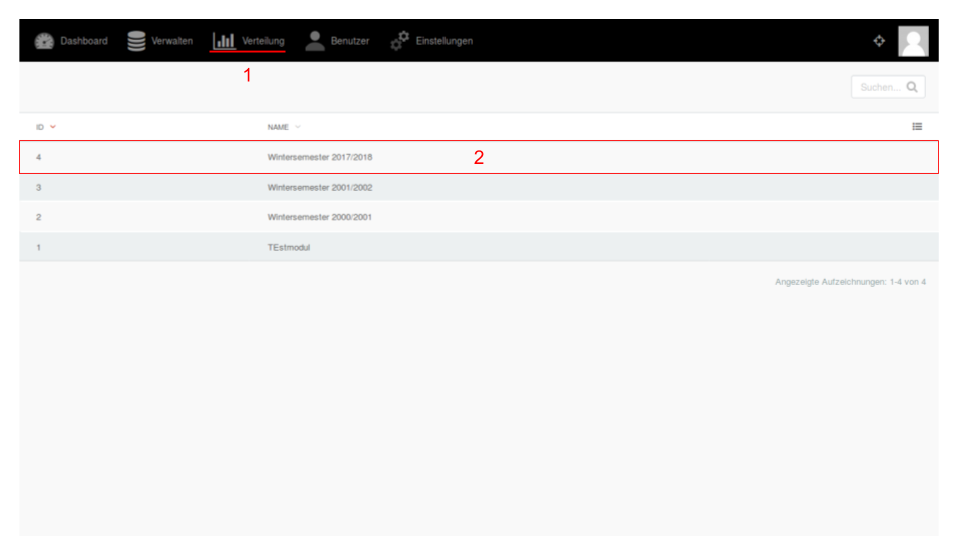
\includegraphics[scale=0.3]{backend/img/distribution_1.png}
  
  \begin{enumerate}
   \item Um eine Verteilung berechnen zu lassen, wechselt der Nutzer in der oberen Hauptnavigation zu dem Punkt ''\textbf{Verteilung}''.
   \item Indem der Nutzer auf eine der vorhandenen Module klickt, kann er mögliche Verteilungen der Studenten auf die Kurse generieren lassen.
  \end{enumerate}
  
  \begin{enumerate}
   \item 
  \end{enumerate}

  
  \section{Benutzer}
  \label{section:users}
  
  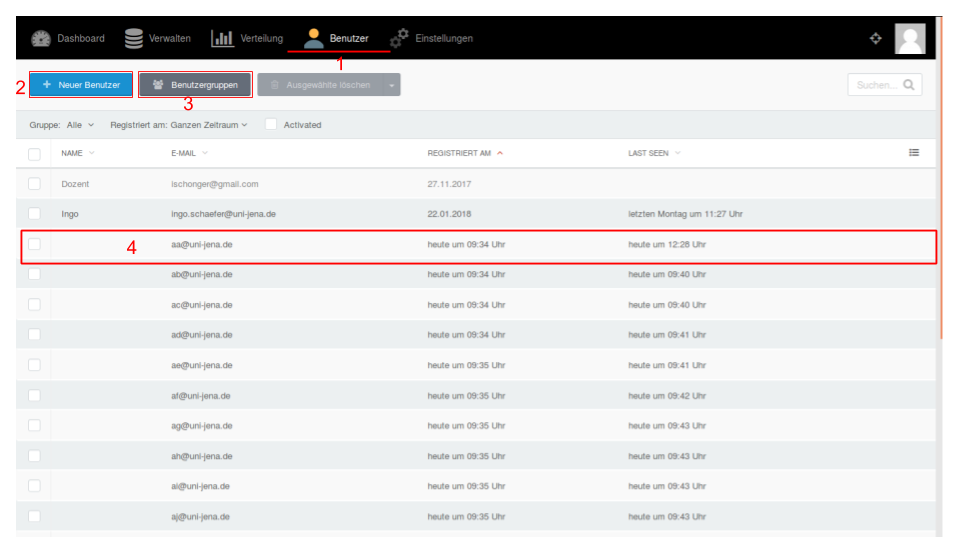
\includegraphics[scale=0.3]{backend/img/users_1.png}
  
  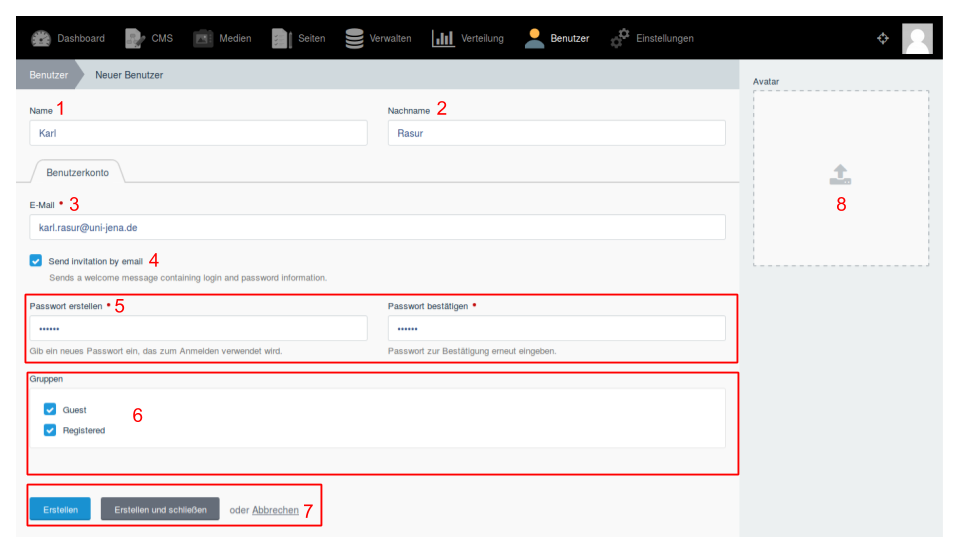
\includegraphics[scale=0.3]{backend/img/neuer_benutzer.png}
    